\documentclass[12pt, a4paper]{book}%, oneside

\usepackage[headings]{fullpage}
\usepackage{setspace}

% \usepackage[top=1.5cm,right=1.5cm,bottom=1.5cm,left=1.5cm]{geometry}
% \usepackage{fancyhdr}
% \setlength{\headheight}{20pt} 
% \usepackage{graphics}
\usepackage{tabularx} % for better control over column width
\usepackage[hyphens]{url}
\usepackage{graphicx}
\usepackage{float}
\floatstyle{plaintop}
\restylefloat{table}
\usepackage{subfig}
\usepackage{array}
\usepackage[table,xcdraw]{xcolor}
% \usepackage{xtab}
\usepackage{multirow}
\usepackage{booktabs}
\usepackage{appendix}
\usepackage[pdfborder={0 0 0}, colorlinks=true, linkcolor=black, citecolor=blue]{hyperref}
\usepackage[printonlyused]{acronym}
\usepackage{algorithmic}
\usepackage{algorithm}
\usepackage{ifpdf}
\graphicspath{{./images/}}
\usepackage{amsmath}
% \setlength{\parindent}{0pt}

\newcommand{\submissionDay}{2}
\newcommand{\submissionMonth}{May}
\newcommand{\submissionYear}{2024}
\newcommand{\submissionDate}{\submissionDay~\submissionMonth,~\submissionYear}
\newcommand{\typeOfThesis}{Bachelor Thesis}

\newcommand{\titleOfThesisOne}{Engineering a Data Benchmark from Textual Posts for Entrepreneurial Personality Analysis}

\newcommand{\authorOfThesis}{Joy Emad Kamel Labib}

\newcommand{\supervisorOne}{Dr. Mervat Mustafa Fahmy Abuelkheir}
\newcommand{\supervisorTwo}{Dr. Nourhan Ehab Abdelhamid Azab}

\newcommand{\includefig}[4]{
    \begin{figure}[ht]
     \centering
      \includegraphics[width=#1\textwidth]{images/#2}
      \caption{#3}
      \label{#4}
    \end{figure}
}

\newcommand{\includefigWSC}[5]{
    \begin{figure}[ht]
     \centering
      \includegraphics[width=#1\textwidth]{images/#2}
      \caption[#3]{#4}
      \label{#5}
    \end{figure}
}

\newcommand{\includeeps}[4]{
\includefig{#1}{#2.eps}{#3}{#4}
}

\newcommand{\includeepsWSC}[5]{
\includefigWSC{#1}{#2.eps}{#3}{#4}{#5}
}


\ifpdf
\pdfinfo {
	/Author (\authorOfThesis)
	/Title (\titleOfThesisOne)
	/Subject (\typeOfThesis)
	/Keywords ()
	/CreationDate (D:20090707085533)
}
\fi

\begin{document}
% \overfullrule=5pt
\pagestyle{plain}
\pagenumbering{Roman}

%\documentclass[12pt]{report}
%\usepackage{graphicx, setspace}

\newcommand{\titlePage}{

\thispagestyle{empty}

\begin{center}
	\textbf{Media Engineering and Technology Faculty}\\[1mm]
	\textbf{German University in Cairo}\\[1mm]
	
\includegraphics[width=2.5cm]{GUC-logo-ss.eps}

	\vspace{2cm}
	\doublespacing
	{\Huge \textbf{Engineering a Data Benchmark from Textual Posts for Entrepreneurial Personality Analysis}}\\
	\singlespacing
	\vspace{2cm}
	{\large \textbf{Bachelor Thesis}}\\

	\vfill
	\parbox{1cm}{
  			\begin{large}
    			\begin{tabbing}
       			Author: \hspace{2cm}  
        			\=\authorOfThesis\\[2mm]
      			Supervisors: 
	      		\>\supervisorOne\\[2mm]
				\>\supervisorTwo\\[2mm]
				\\
				%\>\supervisorThree\\[2mm]
      			Submission Date: 
        			\>\submissionDate\\
    			\end{tabbing}
  		\end{large}
	}\\
\end{center}
\clearpage
}

%\begin{document}

\titlePage
\thispagestyle{empty}
\ \clearpage
\titlePage

\thispagestyle{empty}
This is to certify that:
\begin{itemize}
\item[(i)] the thesis comprises only my original work toward the Bachelor Degree
\item[(ii)] due acknowledgment has been made in the text to all other material used
\end{itemize}

\vspace{2cm}
\begin{flushright}
\rule[0mm]{6cm}{0.2mm}\\
\authorOfThesis\\
\submissionDay~\submissionMonth,~\submissionYear\\
\end{flushright}
\clearpage

%\end{document}


\chapter*{Acknowledgments}
\addcontentsline{toc}{chapter}{Acknowledgments}
\label{chap:ack}
Acknowledgment goes here. 


\chapter*{Abstract}
% \addcontentsline{toc}{chapter}{Abstract}
\label{chap:abstract}
Abstract text goes here.
\tableofcontents
\addcontentsline{toc}{chapter}{Contents}
\clearpage 

\pagestyle{headings}
\pagenumbering{arabic}

% \setlength\parskip{15pt}
\setlength\parskip{.5\baselineskip plus .2\baselineskip
	minus .4\baselineskip}
% \setlength\parskip{.5\baselineskip \@plus .1\baselineskip \@minus ..1\baselineskip}


%\documentclass[12pt]{report}

%\begin{document}

\chapter{Introduction}
\label{chap:intro}
In a fast-paced changing world, where everyone strives to enter the business market and be updated with the latest trends in business, only few people take the risk and start their businesses. Those are called to have an entrepreneurial soul, which permits a person's innovation to have a great impact on the community around them, as well as the economy of their country. 

Defining the word entrepreneur is as simple as describing an instinctive personality filled with identifying opportunities, taking calculated risks, and mobilizing resources. This results in the creation of innovative solutions, products, services, or businesses. Entrepreneurs are characterized by their vision, creativity, resilience, and willingness to positively influence everyone around them.

Since entrepreneurs play a crucial role in driving economic growth and shaping industries through their ability to transform their ideas into real businesses, identifying an entrepreneurial personality becomes more important every day to the economy. It has always been a challenge to recognize the different personalities that exist and define the traits of each one. The entrepreneurial personality is still a complex one, which is linked to a group of specific traits describing the behavior and explaining the decisions they make.

Entrepreneurial personality recognition is currently the concern of various discussions, whether we can classify persons who have an entrepreneurial personality or not. This concerns a lot of businessmen who are willing to invest in small businesses when they don't know whether this person deserves their investment. Additionally, many companies would benefit from such recognition in the recruitment process and selecting the right employee for their industry.

\section{Motivation}
Recognizing a personality depends on identifying the existence of some specific traits with a certain percentage. This inquiry shows these traits through the lifestyle of the person, starting from their daily decisions, their textual posts, the way they communicate with others, and how they approach showing on social media.

As Artificial Intelligence now shaped our usage of technology, it was based on the enormous collected data from diverse resources. This made it possible to train machine learning models that can come up with a clear classification of whether this person has an entrepreneurial personality or not. Unfortunately, no clear standardized dataset was found to train the models, therefore, the classification does not exist yet.

The ability to use text as a main source for this classification, as well as the Artificial Intelligence Analysis would make this classification and help the society to discover the entrepreneurial personalities living within it. This is the main motivation to create such a data benchmark to bring the classification into reality.

\section{Objectives}
The aim of this project is to engineer a data benchmark that can be used to analyze what makes people successful entrepreneurs. This will be done through these objectives:

\begin{enumerate}
\item Investigate diverse sources of textual posts written by entrepreneurs, whether their personal way of expressing themselves in their daily life or the formal way of sharing their experience in life.
\item Extract the textual posts of the entrepreneurs for these sources, accompanied with their meta-data.
\item Design a clear data frame to store all the collected data, along with enriching the data with the textual features for each record.
\item Define a clear pipeline for textual data cleaning from any inconsistencies that could interfere with the classification.
\item Analyze the extracted textual features to reach some validating information of the characteristics that entrepreneurs have in common.
\item Deploy the dataset to be accessible for any consumer working on the analysis of the entrepreneurial personality using a classification of text.
\end{enumerate}

In pursuit of these objectives, our thesis aims not only to contribute to the scholarly discourse surrounding entrepreneurship but also to offer practical insights that may inform and empower aspiring entrepreneurs on their journey to success.

\section{Outline}
This Thesis consists of 5 chapters including the “Introduction”. The second chapter includes the background which explains the entrepreneurial personality and its traits, and examines the role of textual data in personality analysis. It also states the different methodologies used in previous studies and identifying the gaps in current research. The third chapter is the methodology that demonstrates the approach of textual data collection from different sources, the selection criteria, the description of the data processing steps, the labeling of the data, and finally the validation of the dataset. Chapter four represents the findings from the evaluation of the benchmark data set, and the interpretation in the context of existing literature on entrepreneurial personality analysis. As well as, a discussion of the limitations of the study and opportunities for future research. The thesis in concluded in chapter 5 that summarizes the study's contributions to the field of entrepreneurial personality analysis, and a reflection on the importance of standardized benchmarks. It also suggests future directions in the research and implementation of the benchmark.


%\end{document}

% \include{background}
%\documentclass[12pt, a4paper]{book}


%\begin{document}

\chapter{Background}
\label{chap:background}

This chapter includes the background research that founded this bachelor thesis. It is divided into 5 main categories: The Human Personality, The Entrepreneurial Personality, Prediction of the Entrepreneurial Personality, Datasets and lastly, Applications of a Data Benchmark that serves as a high-level introduction to this research.

\section{The Human Personality}
A personality refers to the unique set of individual traits, behaviors, attitudes, and characteristics that distinguish one person from another \cite{kerz2022pushing}. It encompasses the way a person thinks, feels, and behaves across various situations and contexts . Personality is believed to be relatively stable over time but can also be influenced by environmental factors \cite{liao2024open}, experiences, and personal development. Psychologists often study personality to understand how it shapes an individual's thoughts, emotions, motivations, and interactions with others. Personality is closely linked to a broad spectrum of human actions and circumstances, including shopping habits, well-being, social connections, and potentially criminal activities.

The fundamental principle of personality psychology is that stable individual traits lead to consistent behavioral patterns that people tend to show, regardless of the circumstances \cite{vinciarelli2014survey}. Trait models in psychology are constructed based on how people perceive similarities and connections between descriptive words they use to characterize themselves and others. Despite the abundance and diversity of these terms, they generally are reduced  to only a few major dimensions  \cite{vinciarelli2014survey}. 

There are several personality models used in predicting personality, such as Big Five Personality, \ac{mbti} or \ac{disc}. However, after some considerations and literature review process, Big Five Personality is the most popular and precise in telling someone’s personality traits \cite{kerz2022pushing}, \cite{tandera2017personality}. The model describes human personality by five traits/factors, popularly referred to as the Big Five or OCEAN: Openness to experience, Conscientiousness, Extraversion, Agreeableness, and Neuroticism. These traits are today's dominant paradigm in personality research, and one of the most influential models in all of psychology \cite{mccrae2009five}.

%\footnotetext{Normally named Neuroticism, but we will use the inverse stability throughout the paper to ensure consistently positive factor names.}

The Big Five traits are as follows \cite{bacsaran2021neural}, \cite{antoncic2015big}:\begin{enumerate}
\item \textit{Openness to Experience:}\\
Individuals high in openness tend to have broad interests and are often imaginative, creative, and intellectually curious, and may be more receptive to change. However, they may also be prone to overthinking, indecision, and distraction.

\item \textit{Conscientiousness:}\\
Conscientious individuals are characterized by their strong sense of responsibility, self-discipline, and reliability, and also tend to be organized, and detail-oriented. Though, they may be perceived as rigid, perfectionist, and overly cautious.

\item \textit{Extraversion:}\\
Extraverts are sociable, outgoing individuals and derive energy from interacting with others. They tend to be assertive, and often taking on leadership roles \cite{vinciarelli2014survey}. However, they may also experience struggle with introspection, and be prone to risk-taking behaviors.

\item \textit{Agreeableness:}\\
Agreeable individuals are compassionate, empathetic, and cooperative. They tend to be trusting, forgiving and considerate of others' feelings and needs. However, they may also be vulnerable to exploitation, overly trusting.

\item \textit{Neuroticism:}\\
Neuroticism reflects the tendency to experience negative emotions such as anxiety, depression, and moodiness \cite{vinciarelli2014survey}. Individuals high in neuroticism may be prone to worry, and emotional volatility, struggling with feelings of insecurity, self-doubt, and fear of failure.
\end{enumerate}

\section{The Entrepreneurial Personality}
Moving on to a more specific type of personalities that is the focus of this study, which is the entrepreneurial personality. The term "entrepreneur" originates from the French word "entreprendre" and the German word "unternehmen," both of which convey the concept of "undertaking." As per the Webster dictionary, an "entrepreneur" is someone who organizes, manages, and takes on risks of a business or enterprise \cite{singh2013entrepreneurs}. Enterprising behaviour plays an important role in the modern economy which is characterized by instability and rapid change, obliging people and organizations to be in a process of constant innovation \cite{postigo2021general}.

A person may be enterprising at the personal level (personal entrepreneur), which involves demonstrating a strong sense of control and the ability to manage difficult situations and steer their own life \cite{frese20014}. There are two enterprising personalities we can mention, The intra-entrepreneurs and the extra-entrepreneurs. The intra-entrepreneur refers to people who produce changes and innovation within their positions in a company, adding something creative in their projects that are already in progress \cite{mumford2020intrapreneurship}. The extra-entrepreneur is a person whose goal is the development of new external projects and businesses creation \cite{postigo2021general}. The focus of this thesis will be the extra-entrepreneur, or as known as the "general entrepreneur", a person who chooses to work for themselves, not for others.

Additionally, as there are well known standardized traits that measures the different dimensions of a personality, there are specific traits that provides a more precise description of how entrepreneurs and non-entrepreneurs differ in specific behavioral dimensions \cite{postigo2021general}. These traits are measured using the Measure of Entrepreneurial Tendencies and Abilities \ac{meta}, which demonstrated that there is a stronger evidence of predictive accuracy with these traits than the Big Five personality traits. \ac{meta} is a state-of-the-art psychometric test that identifies entrepreneurial potential in order to help businesses nurture and retain their entrepreneurial talent. It assesses four aspects of entrepreneurial personality, namely, entrepreneurial awareness, entrepreneurial creativity, opportunism, and vision  \cite{ahmetoglu2011eq}.

Furthermore, after the development of the \ac{meta}, it was discovered that this measuring instrument has focused on a specific trait in an entrepreneur's personality, so there are no comprehensive, exhaustive, systematic analyses of entrepreneurial personality. Then, new eight dimensions of entrepreneurial personality, for young people and adolescents was developed to include all different aspects \cite{suarez2014screening}. The eight specific traits of an entrepreneurial personality are: 
\begin{enumerate}
\item \textit{Self-efficacy:} 
It refers to a person's ability to organize and carry out actions effectively, and their persistence when encountering obstacles.
\item \textit{Autonomy:}
It refers to the motivation for entrepreneurial creation to achieve a certain individual freedom.
\item \textit{Innovativeness:}
It is the will and interest in finding new ways to do usual daily tasks.
\item \textit{Internal locus of control:}
It is about taking responsibility and attributing the consequences of one's actions to their causes.
\item \textit{Achievement motivation:}
It is the desire to achieve standards of excellence.
\item \textit{Optimism:}
It refers to the beliefs a person has about good things happening more than bad things in their life.
\item \textit{Stress tolerance:}
It can be defined as the resistance to perceiving environmental stimuli as stressors due to the appropriate coping strategies.
\item \textit{Risk-taking:}
It is people's tendency and will to assume certain levels of risk or change to achieve an objective.
\end{enumerate}

Figure~\ref{tab: BigFiveTraits} demonstrates the Big Five Personalities and how can we relate them to the eight specific entrepreneurial traits. As each trait of the Big Five traits can be an umbrella for multiple specific traits. 

\begin{figure}[H]
\centering
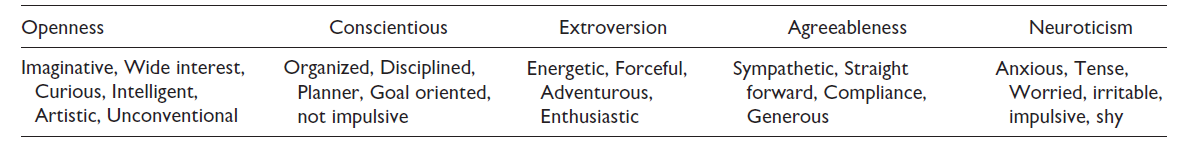
\includegraphics[width=17cm]{Figure1}
\caption{Big Five Personality Traits\cite{suarez2014screening}}
\label{tab: BigFiveTraits}
\end{figure}


\section{Prediction of the Entrepreneurial Personality}
In recent years, there has been a significant evolution in how we approach the analysis and prediction of individuals' personalities. Traditional methods heavily relied on standardized questionnaires and self-report measures. Questionnaires where people rate their own behavior with Likert scales are the instrument most commonly adopted for such a purpose \cite{vinciarelli2014survey}. The most popular questionnaires for predicting the general personality traits include the NEO-Personality-Inventory Revised (NEO-PI-R, 240 items), the NEO Five Factor Inventory (NEO-FFI, 60 items), and the Big-Five Inventory (BFI, 44 items). Short questionnaires (5-10 items), much faster to fill, were built by retaining only those items that best correlate with the results of the full instruments \cite{vinciarelli2014survey}.

Further, for the eight specific entrepreneurial personality traits, the Battery for the assessment of the enterprising personality (BEPE) was developed. The items making up the battery follow a Likert-type format with five answer categories (1 totally disagree, 5 totally agree), in line with established psychometric literature which indicates that between four and six answer categories produce better psychometric indicators \cite{cuesta2018assessment}. The main limitation of self-assessments is that the subjects might tend to bias the ratings towards socially desirable characteristics, especially when the assessment can have negative consequences \cite{vinciarelli2014survey}. 

However, with the rise of technological advancements and social media platforms, there has been a notable shift towards extracting more data from naturalistic data sources. Several works investigate the interplay between personality and computing by measuring the link between traits and use of technology. Online social networks like Twitter, Google+ and Facebook contain much information that can potentially reveal many traits, preferences and opinions of the profile owner. This resulted in research on personal analytic – automatically inferring such latent author attributes in social media \cite{el2022deep}, \cite{tandera2017personality}, \cite{volkova2015inferring}, \cite{vinciarelli2014survey}.

Given its central importance in capturing the essential aspects of human life, increasing attention is being paid to the development of models that can use behavioral data to automatically predict personality. Affective computing focuses on introduces novel techniques that develop and apply affective reasoning tools for personality prediction in multiple modalities and different languages \cite{el2022deep}. They infer personality traits from audio, static image, video, or audio visual clip recorded from various scenarios, such as dyadic dialogue, self-evaluating surveys and self-interviews \cite{liao2024open}. Data obtained from verbal behavior is one of the key types of such data. Even in the early years of psychology, a person's use of language was seen as a distillation of his or her underlying drives, emotions, and thought patterns \cite{kerz2022pushing}. 

With the aid of machine learning models, researchers and practitioners can extract valuable insights from unstructured textual data, such as emails, social media posts, and online forums. By analyzing language patterns, word choices, and linguistic styles, these models can discern underlying personality traits with a higher degree of accuracy than traditional questionnaires \cite{kerz2022pushing}, \cite{volkova2015inferring}, \cite{akrami2019automatic}. These measurements capture the within-text distributions of scores for a given psycholinguistic feature, referred as "text contours". Figure~\ref{fig:featuresALL} lists all features with their examples. There are four main groups for these features  \cite{kerz2022pushing}, \cite{tandera2017personality}, \cite{vinciarelli2014survey}, \cite{el2022deep}:
\begin{enumerate}
\item \textit{Features of morpho-syntactic complexity:}
This group includes surface features such as the average length of clauses and sentences, the features of the type and frequency of embeddings like the number of dependent clauses or the verb phrases, and finally the frequency of particular structure types.

\item \textit{Features of lexical richness, diversity and sophisticated:}
This group includes the lexical density features, like the ratio of lexical words to the total number of words in a text. Also, it includes the lexical variation such as the vocabulary used, the lexical sophistication, for the unusual or advanced words in a text, the psycholinguistic norms of words, and lastly, how much people know this word.

\item \textit{Readability features:}
This group combines a word familiarity variable from a prespecified vocabulary resource, along with a syntactic variable, such as average sentence length.

\item \textit{Lexicon features:}
This last group is derived from a total of ten lexicons that have been successfully used in personality detection, emotion recognition and sentiment analysis research, such as The Affective Norms for English Words (ANEW), DepecheMood++, The \ac{liwc} dictionary, etc \cite{pennebaker1999linguistic}.
\end{enumerate}

\begin{figure}[H]
\centering
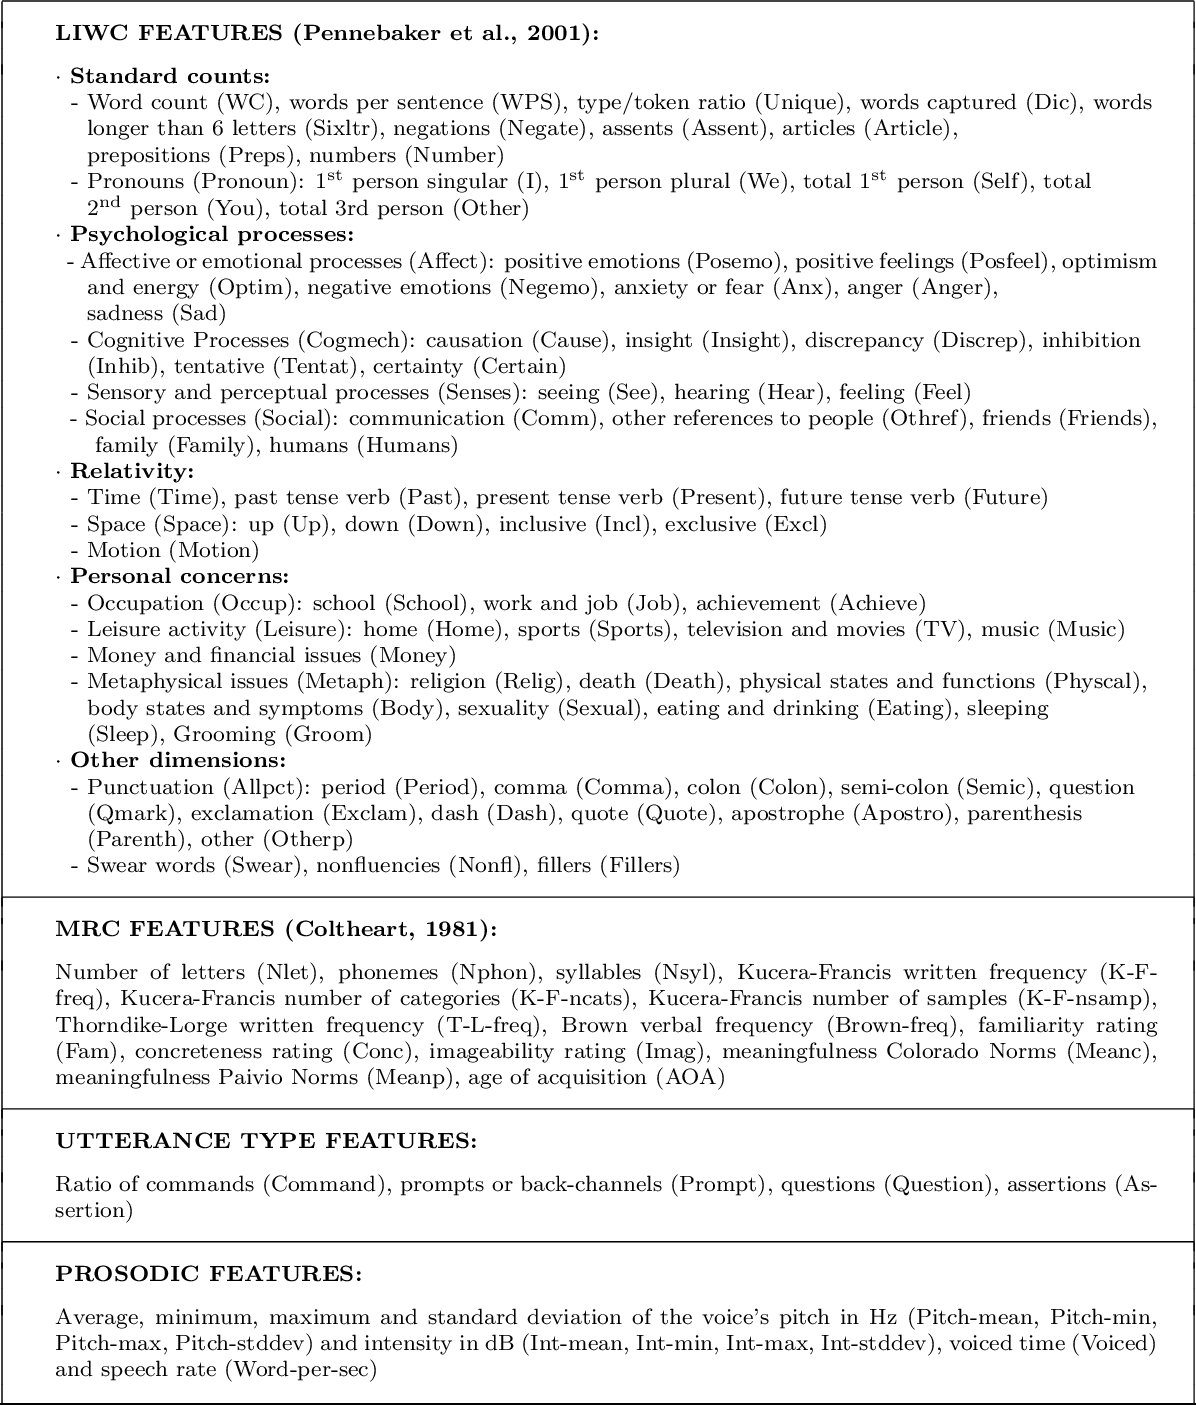
\includegraphics[width=16cm]{LIWC}
\caption{Description of all features, with feature labels in brackets\cite{mairesse2007using}}
\label{fig:featuresALL}
\end{figure}

The aim of this thesis is to gather all the textual characteristics of texts entrepreneurs write and post on their different platforms, and to distinguish if all entrepreneurs write in a unique way, more sophisticated one than non-entrepreneurs.

\section{Datasets}
In order to predict the entrepreneurial personality, and achieve high accuracy in whatever deep learning model used, there has to be a standardized benchmark data to train these models with. Depending on this dataset, the accuracy of the prediction can change and achieving a state-of-the-art models. In this part, we will discover the process of engineering such a dataset, through studying how different benchmark data used to train models to predict the human personality like well-known datasets: The Stream-of-consciousness Essays Database \cite{pennebaker1999linguistic}, myPersonality \cite{kosinski2015facebook}, and built datasets for specific researches.

Starting with the Essays Dataset \cite{pennebaker1999linguistic}, the database encompasses a diverse range of texts, including novels, short stories, and essays, from various literary periods and cultural contexts. On their first Phase, they defined all the reliability of the language use like the text analysis procedures using the \ac{liwc} program, which includes words and categories like emotion category and a sub-category whether it is a negative or positive emotion. Also, they specified the language composition, such as the total number of words, the number of words per sentence, and the number of questions, percentage of unique words, etc. Secondly, they gathered 3 samples of essays from three different sources. The first sample was in a form of daily writings from 15 residential patients in a substance abuse and addiction treatment center in England. The second sample was in a form of daily class assignments by Taos summer school students in New Mexico. The last sample was a group of published abstracts by 40 prominent social psychologists. Each writing sample for each participant was transcribed into a computer text file and analyzed with \ac{liwc} program, and the result is described in figure~\ref{fig:reliabilityStudies}.\\
For their second phase, the 1203 essays were from original psychology student samples as assignments of their fall semester in university. These students also completed occasional questionnaires such as the Five Factor Inventory, these answers were used as a labeling for all the essays. Figure~\ref{fig:LIWCfactors} shows the correlations between the language dimensions and the Five Factor answers. This dataset is considered as a benchmark data, used till this day to train models to predict personality traits.

\begin{figure}[H]
\centering
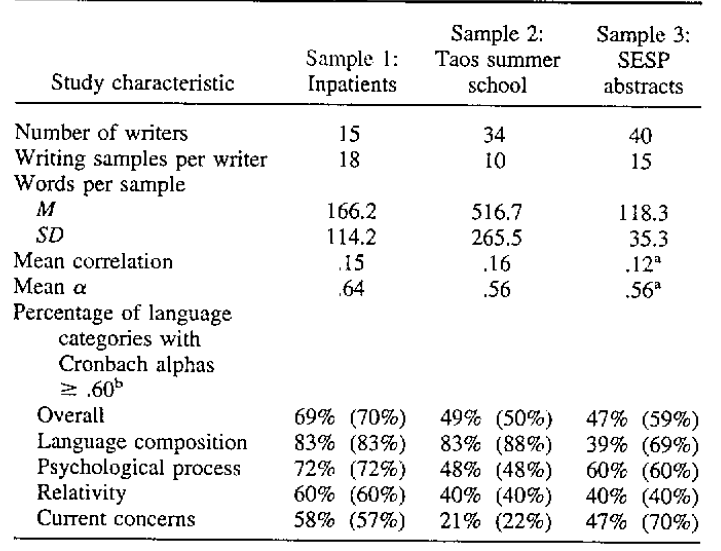
\includegraphics[width=8cm]{Table1}
\caption{Summary of Reliability Studies\cite{mairesse2007using}}
\label{fig:reliabilityStudies}
\end{figure}

\begin{figure}[H]
\centering
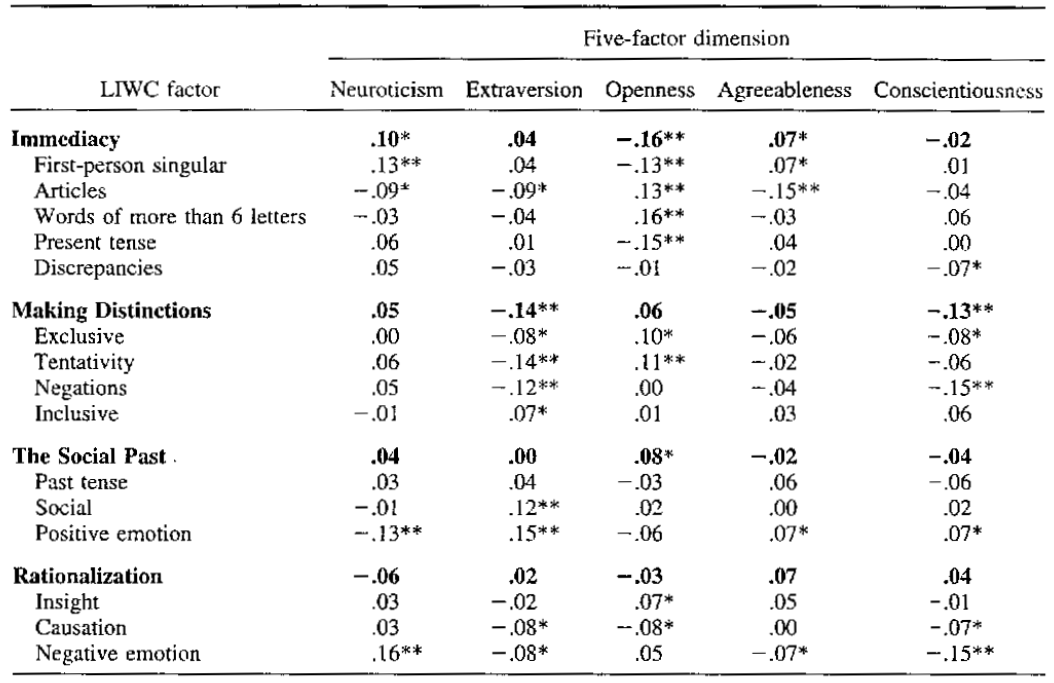
\includegraphics[width=10cm]{Table2}
\caption{\ac{liwc} factors and Simple Correlations With Five-Factor Scores\cite{pennebaker1999linguistic}}
\label{fig:LIWCfactors}
\end{figure}
Furthermore with the myPersonality Database \cite{kosinski2015facebook}, the paper discusses the distinct opportunities and challenges offered by Facebook to researches. It permitted users to complete genuine psychometric assessments and receive immediate results. Alongside test data, approximately 40\% of participants also chose to share information from their Facebook profiles, resulting in one of the largest social science research databases in history. Respondents came from various age groups, backgrounds and cultures. The Database myPersonality offered a 360-degree
assessment feature, encouraging users to invite their friends to judge their personality.  This resulted in a database of cross-ratings,4 while also helping to increase the virality of the application; those who were invited to rate their friends often proceeded to take a test themselves. A sample of how the dataset was build is shown in Figure ~\ref{fig: engineerDataset}. The app remained operational until 2012, amassing data from over 6 million volunteers in 4 years. In April 2018, the researchers decided to stop sharing the data with other scholars. 
\begin{figure}[H]
\centering
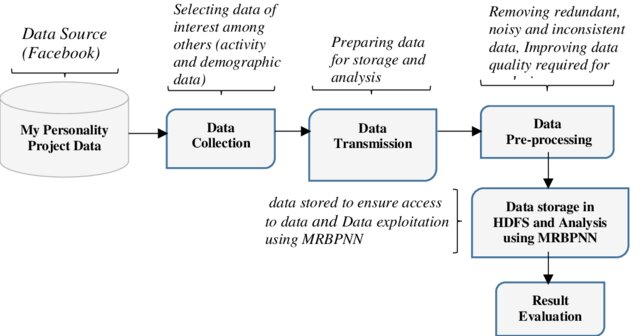
\includegraphics[width=10cm]{Figure3}
\caption{Process to engineering a dataset\cite{kosinski2015facebook}}
\label{fig: engineerDataset}
\end{figure}
Moving on to a database that was built to predict the Big Five personality traits on a scale from -3 to 3, rather than a binary classification \cite{akrami2019automatic}. The researchers required training data, to represent the whole data range for each trait in Swedish language. They proceeded by retrieving data from four different Swedish discussion forums and news sites with authors of different personalities. Web spiders were used to download the texts, and they were 70 million texts in total, but they ended up with only Thirty-nine thousand texts that could be annotated. The texts were annotated by 18 psychology students, each annotated a random text with a specific trait from the Big Five personality traits on a discrete integer interval from -3 to 3 as shown in Figure~\ref{fig: labelsForLargeDataset} . Due to the small number of annotators and the big amount of texts, each text approximately was annotated once. So, it was decided that a smaller subset of the large database would be taken and annotated furthermore, which resulted in a smaller dataset with two thousand texts, with on average 4.5 annotations each as shown in Figure~\ref{fig: labelsForSmallDataset}.

\begin{figure}[H]
\centering
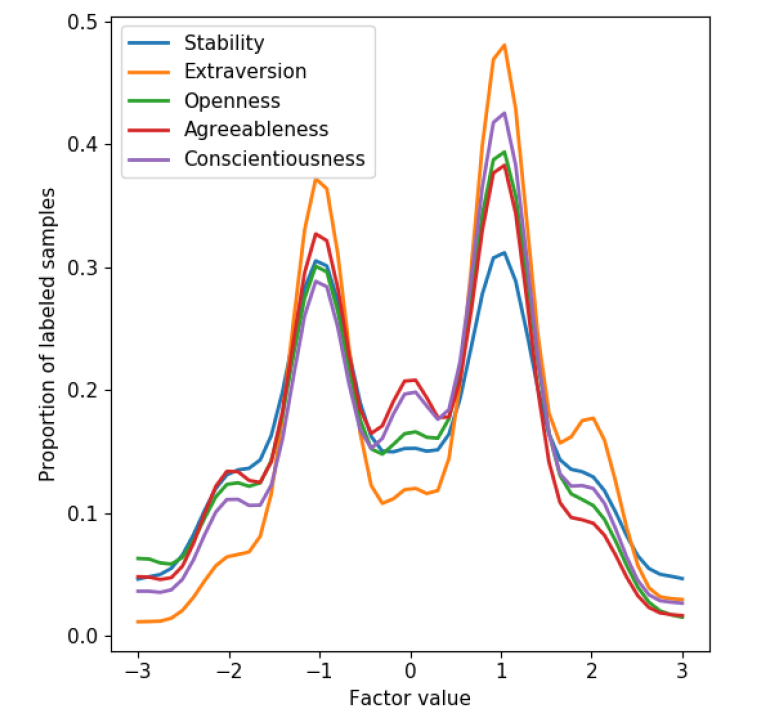
\includegraphics[width=7cm]{Figure4}
\caption{Distribution of labeled samples for each of the factors of the large dataset\cite{akrami2019automatic}.}
\label{fig: labelsForLargeDataset}
\end{figure}

\begin{figure}[H]
\centering
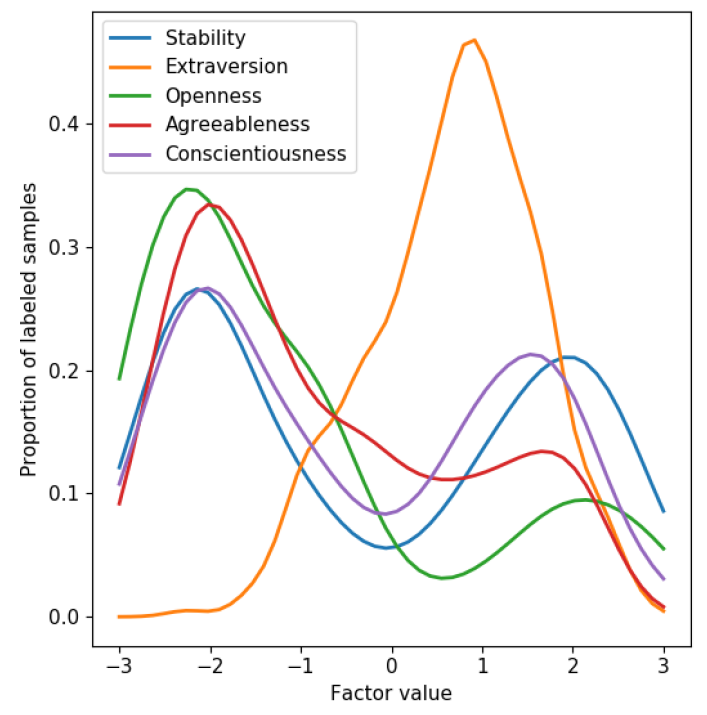
\includegraphics[width=7cm]{Figure5}
\caption{Distribution of labeled samples for each of the factors of the small dataset\cite{akrami2019automatic}.}
\label{fig: labelsForSmallDataset}
\end{figure}

For feature extraction, ther used Term Frequency-Inverse Document Frequency (TF-IDF) to construct features from labeled data. It was used on word and character level with bi-gram for words and quad-grams for characters. Several regression models were tested, and they used ULMFiT as their \ac{nlp}. The performance of the models was evaluated with 5-fold cross validation test, as well as a binary classification test, and they did test their model on wild data like Cover Letters Dataset and Self-Descriptions Dataset. At the end, they were able to create models with reasonable performance, with accuracy in-line with the state-of-the-art models. And, it was found that using a smaller amount of high-quality training data with multi-annotator assessments resulted in models that outperformed models based on a large amount of solo-annotated data. Their results showed that extracting personality traits from a text remained a challenge.

\section{Applications of The Benchmark Data}
Imagine yourself as a recruiter standing in your company's booth in a career fair, meeting all the undergraduates and the graduates, and you are searching to recruit someone for a position with a high leadership skills, innovative, independent, and most importantly a risk taker. You have a new tool at the reach of your hands, to just let the student write a paragraph about himself, and from this paragraph, you will be provided with a direct response if this person has the potential of being an entrepreneur or not, and a detailed explanation on whether or not he should proceed to the next recruitment phase.

Analyzing a simple textual post or comment to predict of the author has the potential to be an entrepreneur or not, or he is already an entrepreneur and owns a business, would be a great asset for companies, for a country's economy and for this person's own self-development. Predicting the entrepreneurial personality can have several application and benefits. Firstly, in the realm of recruitment and selection, companies can harness personality assessments to pinpoint individuals possessing traits conducive to entrepreneurship. By identifying candidates with characteristics such as risk-taking propensity, creativity, and proactiveness, organizations can assemble teams better equipped to innovate and drive business growth \cite{el2022deep}. 

On an individual level, personality assessments provide valuable insights into one's entrepreneurial strengths, weaknesses, and areas for development. By understanding their entrepreneurial personality profile, individuals can focus on honing relevant skills and attributes to enhance their chances of success in entrepreneurial endeavors. Also, it can help social network users to understand how others may perceive them based on how they communicate in social media, in addition to its evident applications in online sales and marketing, targeted advertising, large scale polling and healthcare analytics \cite{volkova2015inferring}.

Similarly, organizations providing business incubation and support services to start-ups can utilize personality assessments to tailor their assistance to the specific needs of entrepreneurs. By understanding the personality profiles of their clients, these organizations can offer targeted mentoring, resources, and networking opportunities to support the start-ups' entrepreneurial journey and maximize their chances of success \cite{antoncic2015big}.

Lastly, at a broader level, policymakers and economic development agencies can leverage personality analysis to understand the entrepreneurial culture within a region or community. By identifying individuals with entrepreneurial potential and providing support and resources to foster their endeavors, policymakers can cultivate a vibrant entrepreneurial ecosystem conducive to economic development and job creation. Policy-makers might like to consider promoting and enhancing entrepreneurship predictive personality factors (particularly openness) early on in the education system among children, teens and students who have the potential to become entrepreneurs \cite{antoncic2015big}.

%\bibliographystyle{ieeetr}
%\bibliography{citations.bib}

%\end{document}

% add more chapters here
\chapter{Methodology}
\label{chap:method}
Engineering a data benchmark has been always a confusing challenge to achieve due to the fact of multiple pipelines to be followed and the different structures of the data. The aim of the thesis is to engineer a data benchmark of textual posts, written by entrepreneurs in different industries. For the purpose of this paper, an entrepreneur is a person who founded a completely independent company, whether on his own or having a co-founder, most importantly, he is working for himself. The benchmark will be a useful tool for the analysis of the entrepreneurial personalities among our communities, through the prediction of the machine learning models. This prediction will be a great asset on the personal level of the person to be an entrepreneur and be validated to have the entrepreneurial characteristics as mentioned before. Though, this prediction is crucially important for the companies looking for the right person with an independent mindset that will help the company reach a new limit for its target, which will indirectly have an impact on the country's economy.

\begin{figure}[H]
\centering
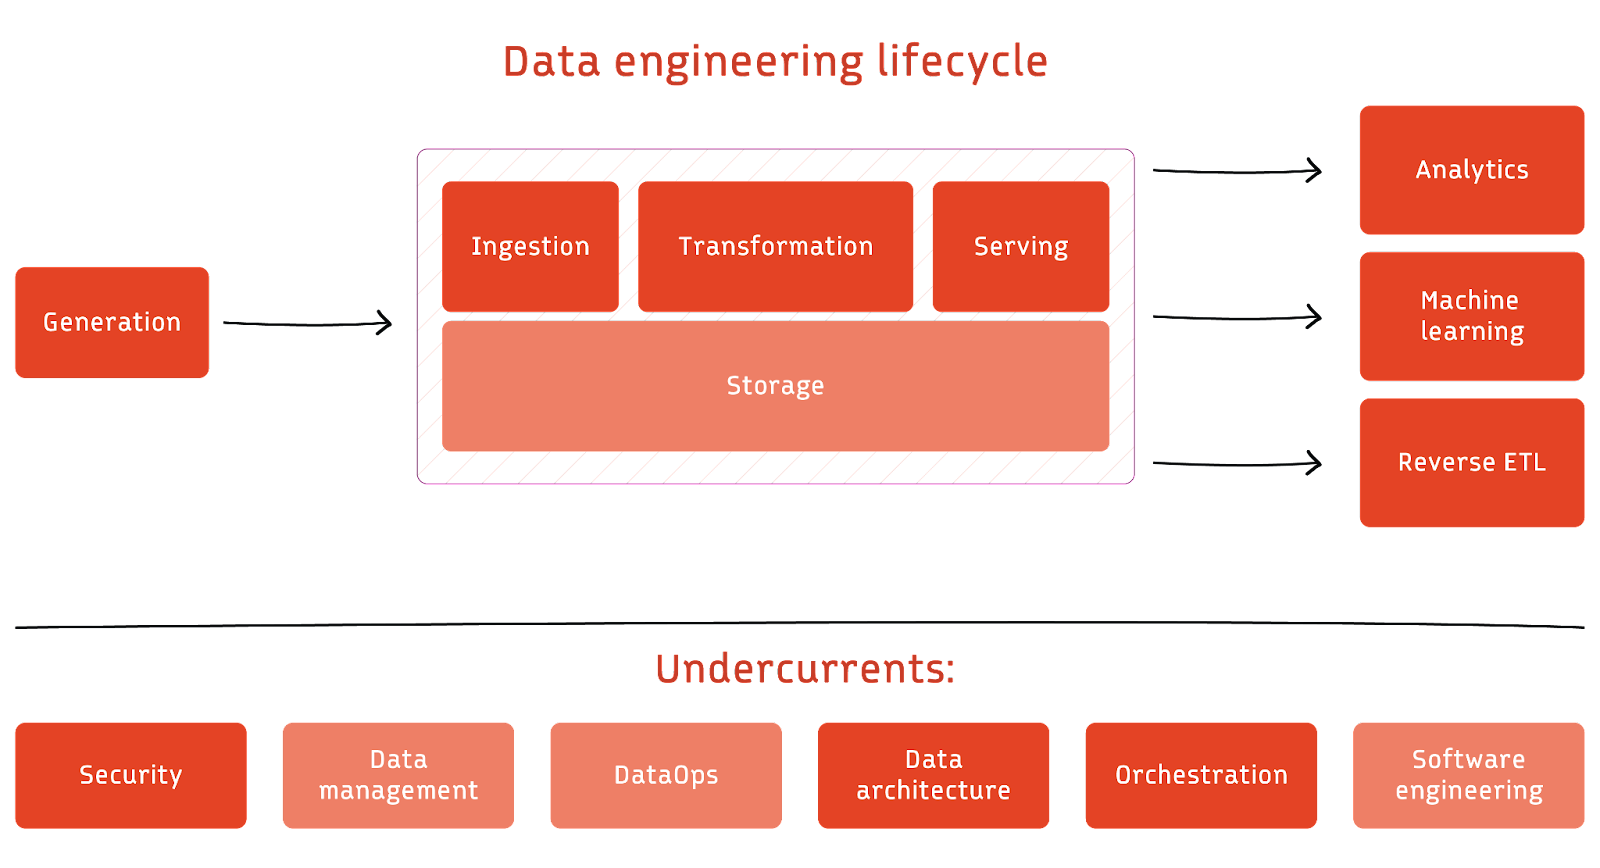
\includegraphics[width=13cm]{datalifecycle}
\caption{Data Engineering Pipeline \cite{Redpanda}}
\label{fig:DataPipelineArchitecture}
\end{figure}

Building a dataset requires to follow a particular process as shown in figure~\ref{fig:DataPipelineArchitecture} from the two different processes \ac{etl}, \ac{elt}, and figure~\ref{fig:etlVselt} illustrates the difference between the two processes. The one used in this thesis is the \ac{elt}, extracting the relevant information needed and transform this data through cleaning and labeling to be more relevant to the thesis' aim. And finally, to validate this data and load it and make it accessible for those who will need it. This chapter includes the different phases followed and the methodology to achieve results in my bachelor thesis. It is divided into 5 main categories: The Data Collection, The Data Transformation, The Textual Features Extraction, The Data Labeling, The Data Validation, and lastly, The Deployment of the data.

\begin{figure}[H]
\centering
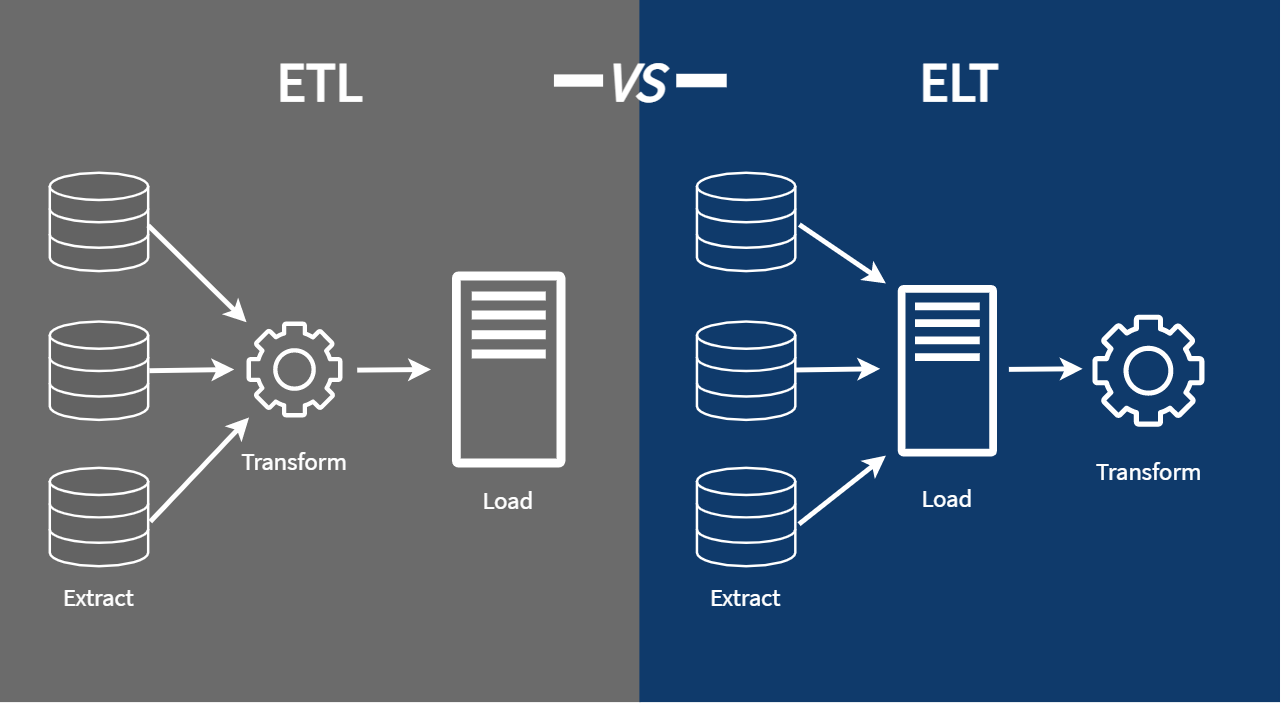
\includegraphics[width=10cm]{etlVSelt}
\caption{Difference between \ac{etl} and \ac{elt} \cite{Leong_2023}}
\label{fig:etlVselt}
\end{figure}

\section{The Data Collection}
The data collection phase is divided into three main parts, according the pipeline followed in this thesis. A research was done to investigate the possible sources of the textual data by entrepreneurs. Afterwards, specifying all the entrepreneurs which will use their texts as the main source of our data, and lastly extracting these texts using various tools.

\subsection{The sources of data}
In contemporary times, anyone can write whatever comes their mind on whichever platforms they prefer on the Internet and publish it to reach the biggest audience. Unfortunately, not all platforms are trustworthy of the published texts and can give multiple false data to the researchers. The investigation of the sources of data phase is a very crucial step to maintain a high quality and comprehensive dataset.

While exploring the different platforms on the Internet that offers people to post their writing and express their opinions for specific topics or for the humanly right for freedom, an important consideration was maintained is to find sources that offers two types of textual posts for our entrepreneurs. The first type focused on the use of the free speech of the entrepreneurs through their social media accounts and the conducted interviews done to discuss their daily lifestyle and their companies establishment journey. The second type focused on the formal use of language through typed articles and blog posts, where entrepreneurs share some advice, lessons learned through their journey to success, and their thoughts on specific topics regarding the industry of their business, or on the general business insights. Having both types of written data is a major key for the entrepreneurial personality analysis, since humans always use the two types on a daily basis, and both types reflect the author's personality characteristics.

After conducting a research on which platforms entrepreneurs usually use to express themselves, several sources and websites \cite{obschonka2017using},  were found to publish entrepreneurs' written contributions. For the free speech textual data type, three main sources were used:

\begin{enumerate}
\item \textbf{X (previously Twitter)}: It is a free social networking site \cite{kwak2010twitter} where users broadcast short posts known as tweets. These tweets can contain text, videos, photos or links. Twitter is known to be the platform where entrepreneurs can build and market for their brand, engage with customers, network with industry professionals, and most importantly stay updated on trends.

\item \textbf{LinkedIn}: It is the world's largest professional network on the internet. It is used to find the right job, connect and strengthen professional relationships, and learn the skills needed to succeed in a career. Entrepreneurs use it as a networking, personal branding, content marketing, industry insights, and partnership opportunities \cite{reed2018linkedin}, \cite{ioanid2015managers}.

\item \textbf{Mixergy}\footnote{\url{https://mixergy.com/}}: Founded by Andrew Warner in 2006, Mixergy offers a variety of content formats, including courses, podcasts, and an extensive library of interviews with founders, CEOs, and other influential figures in the business world.
\end{enumerate}

Furthermore, the formal well-structured posts from entrepreneurs were drawn out from these four sources:
\begin{enumerate}
\item \textbf{The Entrepreneurs Library}\footnote{\url{https://www.theelpodcast.com/}}: It is a podcast, blog, and community for Business proprietors and individuals engaged in small-scale enterprise who loves to read books.
\item \textbf{Entrepreneur Media}\footnote{\url{https://www.entrepreneur.com/}}: It is a multimedia company that provides content, resources, and support for entrepreneurs and small business owners.
\item \textbf{StartupNation}\footnote{\url{https://startupnation.com/}}: Founded by Jeff Sloan, a multimedia company crafted by entrepreneurs for entrepreneurs, offering necessary insights for personal growth.
\item \textbf{Seth's Blog\footnote{\url{https://seths.blog/}}}: The personal blog of Seth Godin, he is a prominent figure in the fields of marketing, entrepreneurship, and leadership.
\end{enumerate}

After an exhaustive research on the sources of texts that will be used for the dataset. We gather all the websites \ac{url}(s) in a Google Sheet, with all the sub-pages that will be accessed to collect the data, too. Putting all the \ac{url}(s) in a data sheet will ease our automation process of transforming the rows of the sheet to a list, separated with commas, which will be used to loop on the list and access the content of each webpage. For example, we created two sheets, one for the list of all entrepreneurs we will extract their LinkedIn posts or their tweets from X (known as Twitter). The other sheet has all the specific webpages of a given website that will be accessed individually with the format of its pagination.

\subsection{Web Scraping}
Web scraping \cite{khder2021web} is a technique used to extract data from websites. As shown in figure~\ref{fig: webscraping} It involves automated processes that navigate through web pages, gather information, and store it for analysis or other purposes. When applied to a list of web pages, web scraping can efficiently collect all the needed data across multiple sites. By writing scripts or using specialized software, users can specify the data they want to extract, such as text, images, or links, and define the pages to scrape. This method is particularly useful for tasks like market research, competitive analysis, and data aggregation, as it allows users to gather large amounts of information quickly and systematically. Additionally, web scraping can be customized to extract structured data from unstructured sources, making it a powerful tool for extracting insights from the vast expanse of the internet.

\begin{figure}[H]
\centering
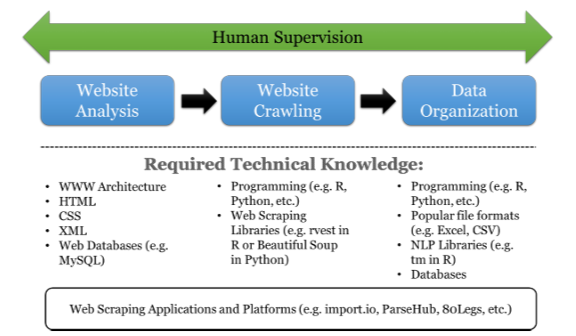
\includegraphics[width=12cm]{webScrapeProcess}
\caption{Web Scraping Process \cite{khder2021web}}
\label{fig: webscraping}
\end{figure}

For each website in our sources, a Python Jupyter Notebook was created using its relative Python packages to extract the data as mentioned in table~\ref{tab:pythonLibraries}. The choice of these libraries depended on the source and the way we want to deal with it to be able to extract all data. For Twitter, it was straight forward to use \textit{Nitter Scraper} since it is an open-source alternative for Twitter where the tweets of a user are seen and iterated through each page without any authentication. For LinkedIn, it wasn't the same easy case like Twitter, we used a webdriver to control the webpage with our code to natigate through the pages and buttons and get the results we want. And finally, for all the other websites, we used requests to access the \ac{url} and get their \ac{html} page source.

\begin{table}[!ht]
    \centering
    \begin{tabular}{|c|c|}
    \hline
        Source & Python libraries\\ \hline
        Twitter & Nitter Scraper (ntscraper), Pandas \\
        LinkedIn & Selenium, BeautifulSoup, Pandas \\
        Other & Requests, BeautifulSoup \\ \hline
    \end{tabular}
    \caption{Sources and their respective Python Libraries}
    \label{tab:pythonLibraries}
\end{table}

Starting of with Twitter, figure~\ref{fig:twitter} below shows the simple python function used to extract all the tweets of a given username to the function responsible for fetching all the data. Along with specifying the fields necessary to form the meta data about our tweet as mentioned in the figure, we construct a dataframe to gather all data and structure it in a tabular form.

\begin{figure}[H]
\centering
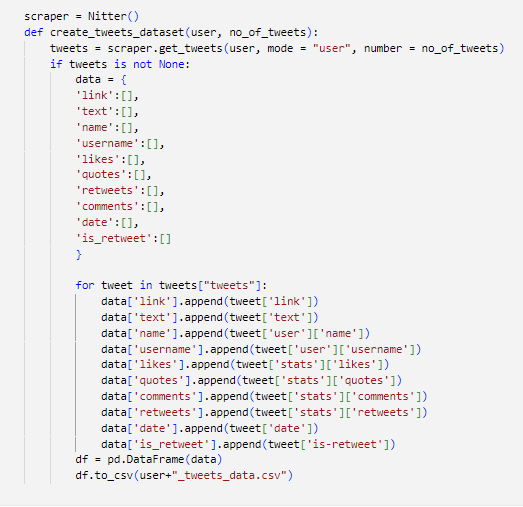
\includegraphics[width=10cm]{twitter}
\caption{Twitter Scraping function using Nitter}
\label{fig:twitter}
\end{figure}

Moving on to LinkedIn, the process of posts extraction is done through two main libraries, Selenium is a powerful tool for automating web browsers. It allowed us to interact with LinkedIn in the same way a user would, and BeautifulSoup to parse the \ac{html} and \ac{xml} documents to extract HTML elements as demonstrated in figure~\ref{fig:linkedin}.

\begin{figure}[H]
\centering
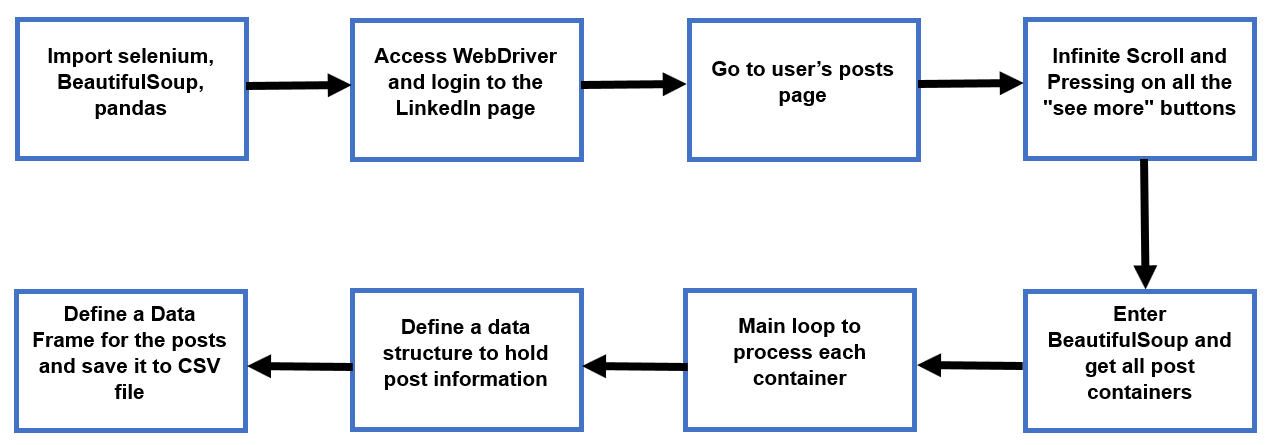
\includegraphics[width=14cm]{LinkedIn}
\caption{LinkedIn Scraping Process}
\label{fig:linkedin}
\end{figure}

At last, all the other sources only needed a great depth inspection to the \ac{html} page source to be able to get all the \ac{html} elements we are interested in, along with their class names, and a unique identifier to collect all the instances of the wanted elements in a page.

\section{The Data Transformation}
Data Transformation is our next step in the data analysis process, aimed at improving the quality and reliability of datasets. It involves integrating the different \ac{csv} files together, to come with one file, and begin the cleaning phase with all its modifications and replacemets within the data to reach a well-balanced and structured dataset.

\subsection{Data Integration}
A dataset has to have one structure for all the derived data from the different sources, that by default has different field names for our records. First of all, we defined a clear structure and the name of fields and its type which we want to appear in the final version of the data benchmark. Afterwards, we order and name all the \ac{csv} file headers with the same name specified earlier. Then, we add a column for each source's \ac{csv} file with the name of the source that the data was collected from to ensure that while cleaning the data, it would be easier to filter the sources and do a true inspection of the data. And the last step, we will gather all the files in one Excel Sheet with all the data from the various sources. The last step is very important, since transforming and cleaning the data phase should be done once for all the data. Skipping this step will require doing the data cleaning on each \ac{csv} file produced from each source, each is very time consuming to do.

\subsection{Data Cleaning}
Data cleaning is a critical prerequisite for any meaningful data analysis and plays a fundamental role in ensuring the reliability and validity of findings in various fields. It involves identifying and correcting errors, inconsistencies, and inaccuracies within the data to ensure its integrity and usefulness for analysis. By conducting thorough data cleaning, analysts can avoid the risk of drawing incorrect conclusions or making flawed decisions based on flawed data. The data cleaning steps starts with an inspection of all the possible errors existing, then the actual cleaning.
\subsubsection{Inspection}
The inspection of data involves detecting the presence of any errors within the \ac{csv} file, which is done using Microsoft Excel automatically. The error can be a result of a non-consistent record value with the auto-generated type of the column by Excel. It draws our attention to any issues in the actual data before starting the cleaning process.

\subsubsection{Cleaning}
This step targets specifically the textual post, not the meta data and the other columns we have in the dataset. It includes a number of modifications to be done on the whole dataset as well as on the text, which will make it more readable and relevant to our dataset definition. These modifications are done through Microsoft Excel and Python libraries as Pandas and NumPy, and they are:
\begin{enumerate}
\item \textbf{Missing Data Handling}\\
Missing values are data points that are absent for a specific variable in a dataset. They can be represented in various ways, such as blank cells, null values, or special symbols like "NA" or "unknown". There are a lot of strategies for missing values, like simply removing the whole row with a missing value, by imputation methods or by the forward or backward filling. We will use the mean imputation method to avoid reducing the sample size or losing the accuracy of the data and introducing certain bias. We filter the texts of the same author and get the mean of any numerical missing values to get the missing one. The figure~\ref{fig:meanImputation} shows an example of doing such a technique with is done with the following formula: 
\[ Mean Value = \frac{\sum_{i=1}^n P_i}{n} \]
where \( P_i \) is the value of an i cell and n is the total number of values.\\
For the textual posts from the sources that hadn't any numerical meta data, we inserted a default value "N/A", to specify that these texts didn't have a count for readers' reactions.
\begin{figure}[H]
\centering
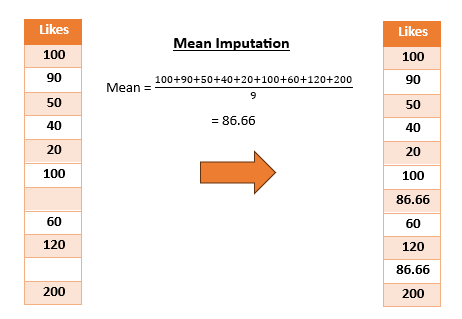
\includegraphics[width=10cm]{meanImputation}
\caption{Example of mean imputation on the likes column}
\label{fig:meanImputation}
\end{figure}

\item \textbf{Duplicates Removal}\\
It is very possible to have a lot of duplicate rows in any dataset, even if is collected through an automated process. Removing duplicates from a dataset ensures data integrity and quality, optimizing storage, and facilitating more accurate analyses. This process enhances overall efficiency and reliability in data management and analysis. Microsoft Excel has a function that can be called on any number of rows and it automatically removes duplicates in our data. The duplicates removal was done based on the textual post only, not any other field, as it has to be the only unique value, at least within all the texts of the same author. As illustrated in figure~\ref{fig:duplicate}, the cells with the same color represents the same content, so we removed the same color cells for each author.
\begin{figure}[H]
\centering
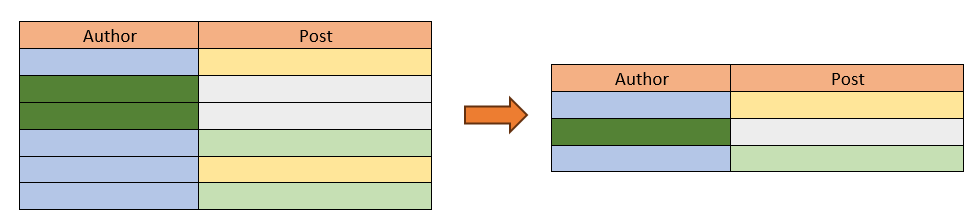
\includegraphics[width=10cm]{duplicates}
\caption{Example of Removing Duplicate Posts}
\label{fig:duplicate}
\end{figure}

\item \textbf{Irrelevant Data Removal}\\
For the entrepreneurial personality analysis, it is very important to have some criteria on the text, to be able to reach validated insights on the data. After a deeper looking into the length of the text that could be analyzed, we came to a conclusion that any text cell value having a number of characters less than 35 characters, the whole row shall be removed. This will be done with Microsoft Excel after adding a column for the length of each text record and removing the rows that applies. 

\item \textbf{Data Type Conversion}\\
Microsoft Excel has an auto-detection of the data type in a column based on the type of the majority of the value. Normally, it directly assigns the type Number to any numerical value, and a string to any textual value. When, it comes to dates, it has only some acceptable formats to write a date, and all the values on a column should hold the same date format, so it is a crucial step to insure that all the dates are written in the same way as depicted in figure~\ref{fig:dateConversion}.
\begin{figure}[H]
\centering
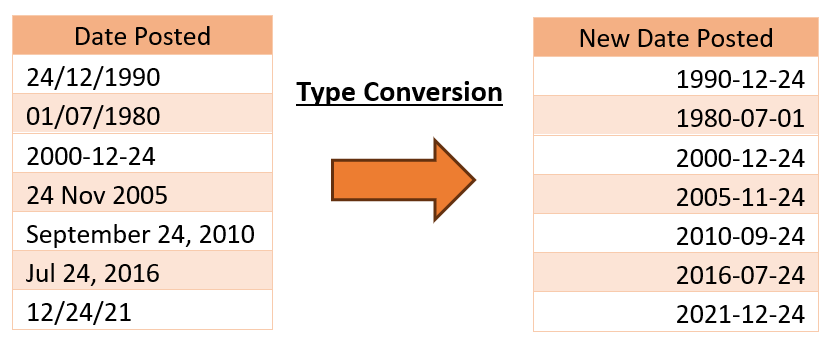
\includegraphics[width=10cm]{dateConversion}
\caption{Example of Date Format Conversion}
\label{fig:dateConversion}
\end{figure}

\item \textbf{Language Translation}\\
To have consistent data, we need to have everything in the same language, because the \ac{nlp} models that analyzes the data are monolingual, they don't process multiple languages at once. We choose English to be our main language. As their are entrepreneurs all around the world, so their was some posts written in Indian and Spanish and other languages. So the languages that we were able to translate to English, we definitely did and for those who we couldn't we had to remove these records.

\item \textbf{Replacing Emojis and Special Characters}\\
Since our data has a lot of free speech textual posts like tweets. Emojis frequently appear in tweets, adding expressive elements to messages and enhancing communication on social media platforms. Unfortunately, emojis can produce unreliable data analysis, and we can't just remove them because nowadays, people tend to express their feelings using emojis since it is easier. Using Demoji library from Python, emojis will be replaced by their textual meeting as illustrated in figure~\ref{fig:emojis} to keep what the entrepreneur really intended to tweet and helps us analyze better their personality characteristics.
\begin{figure}[H]
\centering
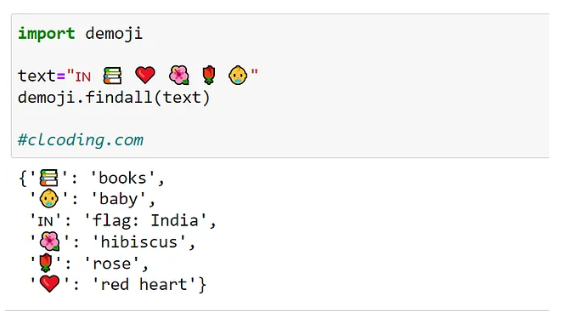
\includegraphics[width=10cm]{emojis}
\caption{Example of Emoji Replacement\cite{SarahDev_2023}}
\label{fig:emojis}
\end{figure}
\end{enumerate}

Minimal cleaning was done on the textual posts, we avoided modifying the text or any specific pre-processing data method to ensure that the text remains in its original format with all the punctuation and the capitalization. The original form will be more useful in the data analysis and the feature engineering of the text that will be later used in the author's personality analysis.

\section{Textual Features Extraction}
Textual features encompass various attributes and characteristics present within written content, serving as key elements for analysis and interpretation. Figure~\ref{fig:features} illustrates the two main branches of the textual features, and we extracted some of the elements of both\cite{litvinova2016profiling}.

\begin{figure}[H]
\centering
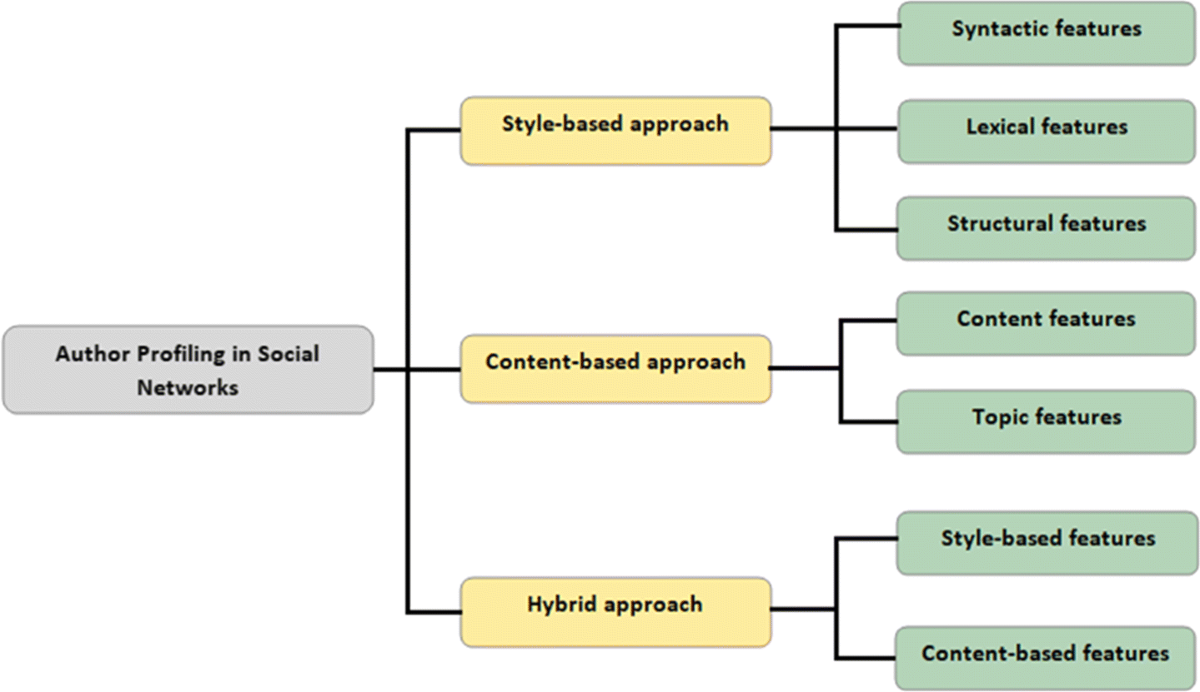
\includegraphics[width=13cm]{features}
\caption{Text Analysis}
\label{fig:features}
\end{figure}

\subsection{Content-based Features}
In \ac{nlp}, feature extraction \cite{tabassum2020survey} is a fundamental task that involves converting raw text data into a format that can be easily processed by machine learning algorithms. There are various techniques available for feature extraction in \ac{nlp}, each with its own strengths and weaknesses. There are multiple available techniques and each has a different use case as demonstrated in table~\ref{tab:featuresExtraction}. After studying each use case for the mentioned techniques, we will be applying the CountVectorizer technique, which will provide us with enough information on the most used words in each text or in the whole \ac{csv}. This technique will be applied using Python, as captured in figure~\ref{fig:CountVectorizer}.

\begin{figure}[H]
\centering
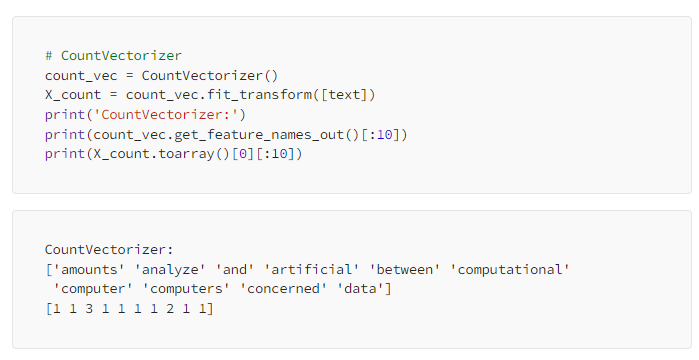
\includegraphics[width=15cm]{CountVectorizer}
\caption{Example of CountVectorizer with Python\cite{Eskandar_2023}}
\label{fig:CountVectorizer}
\end{figure}

The application of CountVectorizer in our case, is to have the words with the biggest number of occurrences within a text. Therefore, the returned words will help to better understand the most used words by entrepreneurs.

\begin{table}[H]
\caption{Comparison of Text Feature Extraction Techniques\cite{Eskandar_2023}}
\label{tab:featuresExtraction}
\begin{tabular}{m{7em}m{10em}m{7em}m{12em}}
\hline
\textbf{Technique} &
  \textbf{Main Features} &
  \textbf{Use Cases} &
  \textbf{Size and Complexity} \\ \hline
CountVectorizer &
  Converts text to Matrix of word count &
  {\color[HTML]{111B21} Text classification, topic modeling} &
  Simple and fast, suitable for small to medium-sized datasets \\ \hline
TF-IDF &
  {\color[HTML]{111B21} Assigns weights towards based on importance} &
  {\color[HTML]{111B21} Information retrieval, text classification} &
  {\color[HTML]{111B21} More complex and computationally expensive suitable for medium to large-sized datasets} \\ \hline
Word embeddings &
  Vector representation of words based on semantics and syntax &
  {\color[HTML]{111B21} Text classification, information retrieval} &
  Can handle large datasets computationally expensive to train \\ \hline
Bag of  Words &
  Represents text as a vector of  word frequencies &
  Text classification, sentiment analysis &
  Simple and fast suitable for small to medium-sized datasets \\ \hline
Bag of n-grams &
  Captures frequency of sequences of n words &
  Text classification, sentiment analysis &
  It depends on the size of the n-grams and the datasets \\ \hline
Hashing Vectorizer &
  Maps words to fixed-size features space using hashing function &
  Large scale text classification, online learning &
  Suitable for large datasets memory efficient May suffered from hash collisions \\ \hline
\end{tabular}
\end{table}

\subsection{Style-based Features}
The style-based features of a text focus on linguistic attributes such as tone, writing style, frequency of use of punctuation, and in case of the tweets, the number of hashtags and emojis. The following list shows all the features we derived from the textual posts, that will be used in the later section:
\begin{enumerate}
\item \textit{Use of Pronouns:} \\
The conversational tone was measured with the frequency of occurrences of specific pronouns and its instances as listed in table~\ref{tab:pronouns}. This feature will be extracted through Python by specifying the pronouns as a dictionary and searching through the CountVectorizer result, we will get the actual frequency.

\begin{table}[H]
\centering
\caption{Pronouns for Tone Analysis}
\label{tab:pronouns}
\begin{tabular}{cccc}
\hline
\textbf{Nominative} &
  \textbf{Objective} &
  \textbf{First Possessive} &
  \textbf{Second Possessive} \\ \hline
I & Me & My & Mine \\ \hline
You & You & Your & Yours \\ \hline
He & Him & His & His \\ \hline
She & Her & Her & Hers \\ \hline
We & Us & Our & Ours \\ \hline
They & Them & Their & Theirs \\ \hline
\end{tabular}
\end{table}

\item \textit{The average word length:}\\
The length of a word tends to determine the tone of the author. As shorter words tends to be punchier and harder, in opposition to longer words that give a softer effect \cite{Baxter-Read_Baxter-Read_2023}. So it will be beneficial to calculate the average word length used in the text through Python.

\item \textit{The average sentence length:}\\
Same as for the word length, the length of a sentence decides the tempo of the long text. Shorter sentences, less than or equals to 10 words give a concise style. While longer ones can be a little confusing.

\item \textit{The text length by word count and sentence count:}\\
Text length can significantly impact communication effectiveness by influencing readability and comprehension. It balances conveying sufficient information without overwhelming the reader. We used Python to count the number of words and number of sentences in the text.

\item \textit{Polarity:}\\
The polarity score is calculated to assess whether the overall text leans towards being positive or negative.
The positive and negative score in calculated based on a positive or negative dictionary that when a word is found the score increase in either side. Table~\ref{tab:negativePositive} shows an example of the negative and positive dictionary. The formula used to compute the polarity score is as follows, illustrated in figure~\ref{fig:subjective}: 
\[ Polarity Score = \frac{Positive Score - Negative Score}{Positive Score + Negative Score + 0.000001} \]

\begin{table}[H]
\centering
\caption{Example of Positive and Negative Dictionary\cite{Mining2017Media}}
\label{tab:negativePositive}
\begin{tabular}{ccc}
\hline
\textbf{Serial No.} &
  \textbf{Positive words} &
  \textbf{Negative words} \\ \hline
1 & Amazing & Avoid \\ \hline
2 & Authentic & Mistakes \\ \hline
3 & Best & Bad \\ \hline
4 & Benefits & Complicated \\ \hline
5 & Better & Error \\ \hline
6 & Great & Fail \\ \hline
7 & Happy & Sad \\ \hline
8 & Inspiring & Unhappy \\ \hline
9 & Productive \\ \hline
10 & Thankful
\end{tabular}
\end{table}

\item \textit{Subjectivity:}\\
The subjective score is used to assess the level of subjectivity or opinion expressed in a text. Figure~\ref{fig:subjective} illustrates the relationship between the polarity and the subjectivity of a text. It is calculated using the formula:
\[ Subjective Score = \frac{Positive Score + Negative Score}{Total Words after cleaning + 0.000001} \]

\begin{figure}[H]
\centering
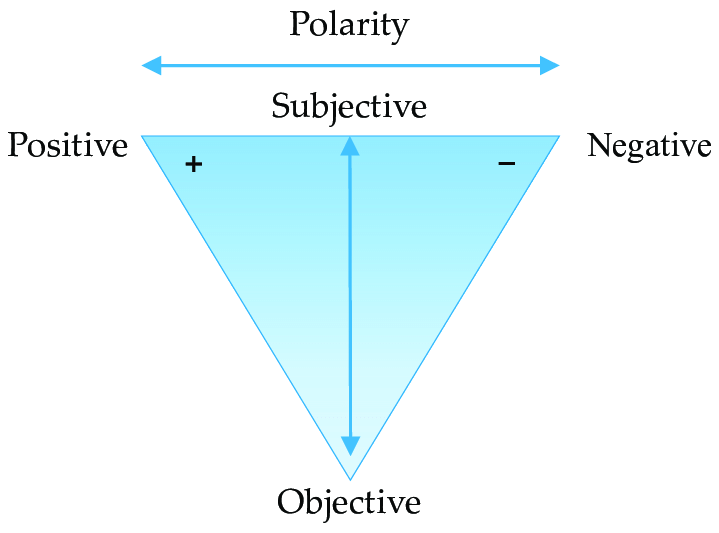
\includegraphics[width=8cm]{Subjective}
\caption{The relationship between Polarity and Subjectivity \cite{Ghani2018}}
\label{fig:subjective}
\end{figure}

\item \textit{Complex Word Count:}\\
The complex word count refers to the number of words in the text that have more than two syllables \cite{Celestial_2023}.Using Python's library \textit{cmudict}, we will build a function that counts the syllables of a word and then check if the word in complex and finally, return the complex words count.

\item \textit{Use of Punctuation:}\\
Punctuation is essential in writing because it helps to convey meaning and clarify the structure of sentences. Without punctuation, sentences can become confusing or ambiguous, making it harder for readers to understand the intended message. Punctuation marks as demonstrated in figure~\ref{fig:punctuation}.

\begin{figure}[H]
\centering
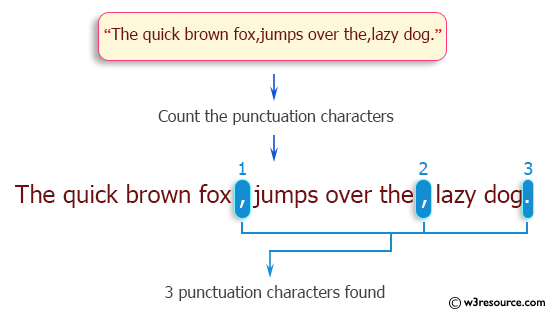
\includegraphics[width=10cm]{punctuation1}
\caption{The punctuation count in a sentence with Python}
\label{fig:punctuation}
\end{figure}

\item \textit{Uppercase and Lowercase words:}\\
Identifying the frequency of the using Uppercase words in opposition to the lowercase words. We will extract two values, one for the whole uppercase words and one for only the words having their first letter an uppercase. And, same goes for the lowercase words.
\end{enumerate}

\section{The Data Labeling}
Data labeling is the process of adding tags or labels to raw data, in our case, the raw data will be the textual posts or tweets of entrepreneurs. Since, the aim of this thesis in to analyze the entrepreneurial personality through verbal behaviour, data labeling will help to come up with conclusions on how entrepreneurs write. And, for future work we wish to be make the prediction if a given textual input has the entrepreneurial personality or not, the labels would represent an object class to help Machine Learning models learn to recognize specific classes within the data without labels.

Using all the extracted features mentioned in the previous section, a column will be made for each feature with the header as the feature name and the value or score it got on this feature. As demonstrated in figure~\ref{fig:labeling} we added to the rows additional information regarding their features.


\begin{figure}[H]
\centering
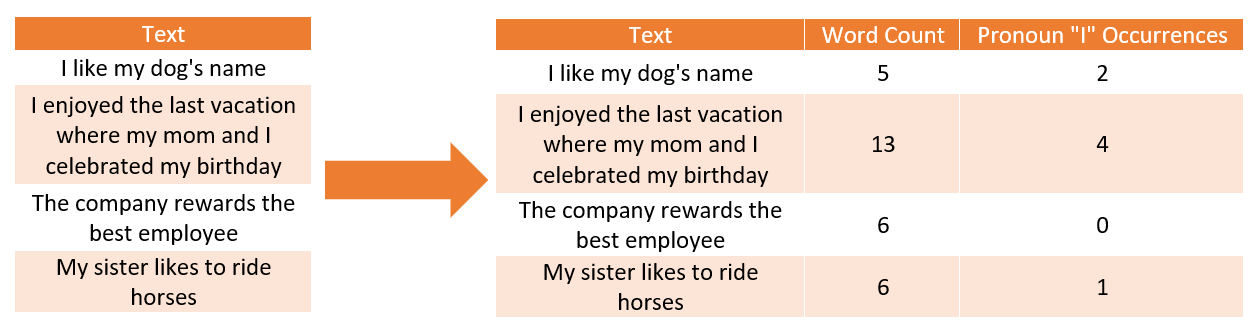
\includegraphics[width=15cm]{labeling}
\caption{Example of data labeling}
\label{fig:labeling}
\end{figure}

Since, the focus of the thesis is about the characteristics of the entrepreneurial personality and this is the first dataset of entrepreneurs' writings, we focus on the \ac{liwc} features more than labeling the dataset with the personality traits of the text. To have a ready dataset as input for the Machine Learning prediction models, we aspire to have a labeled dataset with the Big Five Personality variables or \ac{mbti} variations, to better understand the different aspects of the entrepreneurial personality. Unfortunately, this aspiration is not possible at the moment, since only two state-of-the-art models, the \ac{liwc} and the IBM Watson Personality Insights, offer this feature to extract the personality traits from text. And, these two models have a very limited free access. This task can be done as a new labeled version of this dataset with the traits in the future.

\section{The Data Validation}
To ensure that data is accurate, complete, and consistent, data validation is the necessary process for this step. It involves checking data for errors, inconsistencies, and anomalies to maintain data quality and reliability. This process is crucial, especially when dealing with large datasets, as errors can propagate quickly and impact downstream analyses or decisions.

Data can be examined as part of a validation process in a variety of ways, including data type, constraint, structured, consistency and code validation. Each type of data validation is designed to make sure the textual posts meet the requirements to be useful for analysis.

Among the most basic and common ways that data is used is within a spreadsheet program such as Microsoft Excel or Google Sheets. In both Excel and Sheets, the data validation process is a straightforward, integrated feature. Excel and Sheets both have a menu item listed as Data > Data Validation. By selecting the Data Validation menu, a user can choose the specific data type or constraint validation required for a given file or data range.

Figure~\ref{fig:validation} illustrates the automatic process of data validation that is done. The types of data validation we did on our dataset:
\begin{itemize}
\item \textbf{Data type validation:}\\ It confirms that the data in each field or column matches a specified data type and format.
\item \textbf{Constraint validation:}\\
It checks to see if a given data field input fits a specified requirement within certain ranges. For example, it verifies that a textual post field has the minimum number of characters.
\item \textbf{Structured validation:}\\
It ensures that the data is compliant with the specified data schema we set at the data transformation phase.
\item \textbf{Consistency validation:}\\
It makes sure data styles are consistent. For example, it confirms that all values of the feature extraction scores are listed to two decimal points.
\end{itemize}

\begin{figure}[H]
\centering
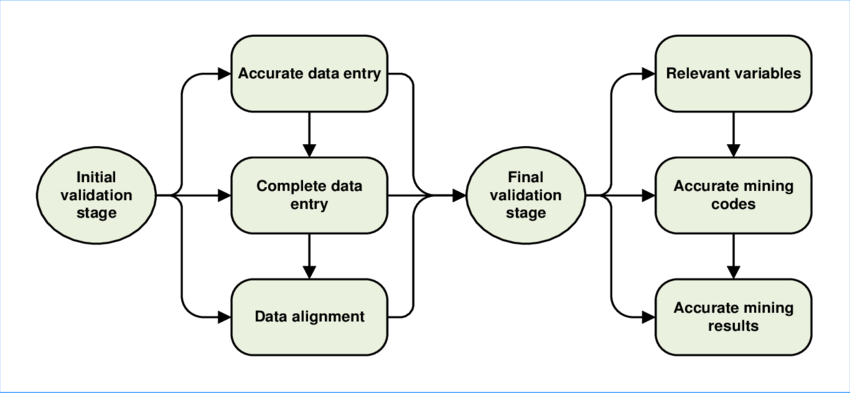
\includegraphics[width=15cm]{validation}
\caption{Data validation process stages\cite{okeowo2018investigating}}
\label{fig:validation}
\end{figure}

The output of any given system can only be as good as the data the operation is based on. These operations can include machine learning or artificial intelligence models, data analytic reports and business intelligence dashboards. These reports and data visualization can be a great asset in validating the data and discover any outliers in the columns.

\section{Data Visualization}
Data visualization is the visual presentation of data or information. The goal of data visualization is to communicate data or information clearly and effectively to readers. The field of data visualization combines both art and data science. While a data visualization can be creative and pleasing to look at, it should also be functional in its visual communication of the data.

Data visualization can be used for:
\begin{itemize}
\item Making data engaging and easily digestible
\item Identifying trends and outliers within a set of data, as mentioned before in the data validation phase
\item Telling a story found within the data
\item Highlighting the important parts of a set of data
\end{itemize}

Data can be represented in a lot of forms, but most importantly, is the choice of the form and how it serves our use case and the data type we want to visualize. Figure~\ref{fig:charts}shows some of these forms in a very artistic way.

\begin{figure}[H]
\centering
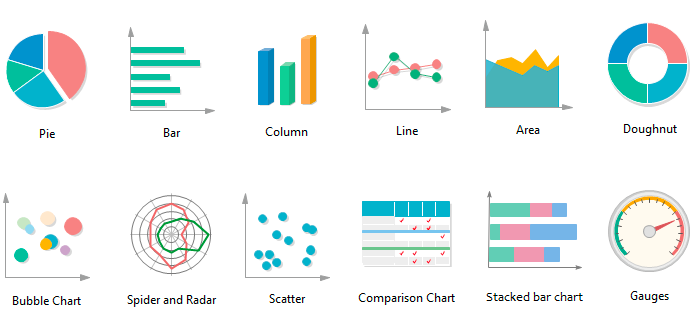
\includegraphics[width=15cm]{charts}
\caption{Data Visualization\cite{Sdhglobal_2023}}
\label{fig:charts}
\end{figure}
\chapter{Results \& Limitations}
\label{chap:result}
\section{Experiments Setup}
Section text.

\section{Dataset Description}
Section text.

\section{Results}
Section text.
\subsection{Experiment 1}
Subsection text. 

\subsection{Experiment 2}
Subsection text.

\section{Results Analysis and Discussion}
Section text.

\chapter{Conclusion \& Future Work}\label{chap:concl}

\section{Conclusion}
Section text.

\section{Future Work}

Section text.
\appendix
\renewcommand{\appendixtocname}{Appendix}
\renewcommand{\appendixpagename}{\appendixtocname}
\addappheadtotoc
\setboolean{@twoside}{false}
\appendixpage

\chapter{Lists}
\addcontentsline{toc}{section}{List of Abbreviations}
\begin{acronym}[\hspace{3cm}]
  \acro{mbti}[MBTI]{Myers-Briggs Type Indicator \cite{kerz2022pushing}}
  \acro{disc}[DISC]{Dominance Influence Steadiness Conscientiousness\cite{kerz2022pushing}}
  \acro{meta}[META]{Measure of Entrepreneurial Tendencies and Abilities \cite{postigo2021general}}
  \acro{liwc}[LIWC]{Linguistic Inquiry Word Count \cite{pennebaker1999linguistic}}
  \acro{nlp}[NLP]{Natural Language Processing}
  \acro{etl}[ETL]{Extract Transform Load}
  \acro{elt}[ELT]{Extract Load Transform}
  \acro{etlt}[ETLT]{Extract Transform Load Transform}
  \acro{url}[URL]{Uniform Resource Locator}
  \acro{html}[HTML]{Hypertext Markup Language}
  \acro{xml}[XML]{Extensible Markup Language}
  \acro{csv}[CSV]{Comma-Separated Values file}
\end{acronym}
\clearpage
\listoffigures
\addcontentsline{toc}{section}{List of Figures}
\listoftables
\addcontentsline{toc}{section}{List of Tables}


\bibliographystyle{plain}
\bibliography{citations.bib}
\addcontentsline{toc}{chapter}{References}

\end{document}
